\subsection{Pocket Rubik's Cube (2*2*2) and SAT solver}
\label{PocketCubeSAT}.

\renewcommand{\CURPATH}{puzzles/rubik2/SAT}

I had success with my SAT-based solver, which can find an 11-turn path for a matter of 10-20 minutes on my old
Intel Xeon E3-1220 3.10GHz.

First, we will encode each color as 3-bit bit vector.
Then we can build electronic circuit, which will take initial state of cube and output final state.
It can have switches for each turn on each state.

% TODO TikZ
\begin{lstlisting}
                 +-----+    +-----+     +-----+
initial state -> | blk | -> | blk | ... | blk | -> final state
                 +-----+    +-----+     +-----+
                    ^          ^           ^
                    |          |           |
                  turn 1     turn 2    last turn
\end{lstlisting}

You set all turns and the device "calculates" final state.

Each "blk" can be constisted of 24 multiplexers (MUX), each for each facelet.
Each MUX is controlled by 5-bit command (turn number).
Depending on command, MUX takes 3-bit color from a facelet from a previous state.

Here is a table: the first column is a "destination" facelet, then a list of "source" facelets for each turn:

\begin{lstlisting}
    #      dst,  FCW  FH   FCCW UCW  UH   UCCW DCW  DH   DCCW RCW  RH   RCCW LCW  LH   LCCW BCW  BH   BCCW
    add_r("F1",["F3","F4","F2","R1","B1","L1","F1","F1","F1","F1","F1","F1","U1","B4","D1","F1","F1","F1"])
    add_r("F2",["F1","F3","F4","R2","B2","L2","F2","F2","F2","D2","B3","U2","F2","F2","F2","F2","F2","F2"])
    add_r("F3",["F4","F2","F1","F3","F3","F3","L3","B3","R3","F3","F3","F3","U3","B2","D3","F3","F3","F3"])
    add_r("F4",["F2","F1","F3","F4","F4","F4","L4","B4","R4","D4","B1","U4","F4","F4","F4","F4","F4","F4"])
    add_r("U1",["U1","U1","U1","U3","U4","U2","U1","U1","U1","U1","U1","U1","B4","D1","F1","R2","D4","L3"])
    add_r("U2",["U2","U2","U2","U1","U3","U4","U2","U2","U2","F2","D2","B3","U2","U2","U2","R4","D3","L1"])
    add_r("U3",["L4","D2","R1","U4","U2","U1","U3","U3","U3","U3","U3","U3","B2","D3","F3","U3","U3","U3"])
    add_r("U4",["L2","D1","R3","U2","U1","U3","U4","U4","U4","F4","D4","B1","U4","U4","U4","U4","U4","U4"])
    add_r("D1",["R3","U4","L2","D1","D1","D1","D3","D4","D2","D1","D1","D1","F1","U1","B4","D1","D1","D1"])
    add_r("D2",["R1","U3","L4","D2","D2","D2","D1","D3","D4","B3","U2","F2","D2","D2","D2","D2","D2","D2"])
    add_r("D3",["D3","D3","D3","D3","D3","D3","D4","D2","D1","D3","D3","D3","F3","U3","B2","L1","U2","R4"])
    add_r("D4",["D4","D4","D4","D4","D4","D4","D2","D1","D3","B1","U4","F4","D4","D4","D4","L3","U1","R2"])
    add_r("R1",["U3","L4","D2","B1","L1","F1","R1","R1","R1","R3","R4","R2","R1","R1","R1","R1","R1","R1"])
    add_r("R2",["R2","R2","R2","B2","L2","F2","R2","R2","R2","R1","R3","R4","R2","R2","R2","D4","L3","U1"])
    add_r("R3",["U4","L2","D1","R3","R3","R3","F3","L3","B3","R4","R2","R1","R3","R3","R3","R3","R3","R3"])
    add_r("R4",["R4","R4","R4","R4","R4","R4","F4","L4","B4","R2","R1","R3","R4","R4","R4","D3","L1","U2"])
    add_r("L1",["L1","L1","L1","F1","R1","B1","L1","L1","L1","L1","L1","L1","L3","L4","L2","U2","R4","D3"])
    add_r("L2",["D1","R3","U4","F2","R2","B2","L2","L2","L2","L2","L2","L2","L1","L3","L4","L2","L2","L2"])
    add_r("L3",["L3","L3","L3","L3","L3","L3","B3","R3","F3","L3","L3","L3","L4","L2","L1","U1","R2","D4"])
    add_r("L4",["D2","R1","U3","L4","L4","L4","B4","R4","F4","L4","L4","L4","L2","L1","L3","L4","L4","L4"])
    add_r("B1",["B1","B1","B1","L1","F1","R1","B1","B1","B1","U4","F4","D4","B1","B1","B1","B3","B4","B2"])
    add_r("B2",["B2","B2","B2","L2","F2","R2","B2","B2","B2","B2","B2","B2","D3","F3","U3","B1","B3","B4"])
    add_r("B3",["B3","B3","B3","B3","B3","B3","R3","F3","L3","U2","F2","D2","B3","B3","B3","B4","B2","B1"])
    add_r("B4",["B4","B4","B4","B4","B4","B4","R4","F4","L4","B4","B4","B4","D1","F1","U1","B2","B1","B3"])
\end{lstlisting}

Each MUX has 32 inputs, each has width of 3 bits: colors from "source" facelets.
It has 3-bit output (color for "destination" facelet).
It has 5-bit selector, for 18 turns. Other selector values (32-18=14 values) are not used at all.

The whole problem is to build a circuit and then ask SAT solver to set "switches" to such a state,
when input and output are determined (by us).

Now the problem is to represent MUX in CNF terms.

From \ac{EE} courses we can remember about a simple if-then-else (ITE) gate, it takes 3 inputs
("selector", "true" and "false") and it has 1 output.
Depending on "selector" input it "connects" output with "true" or "false" input.
Using tree of ITE gates we first can build 32-to-1 MUX, then wide 32*3-to-3 MUX.

I once have written small utility to search for shortest possible CNF formula for a specific function,
in a bruteforce manner (\url{https://github.com/DennisYurichev/SAT_SMT_by_example/blob/master/puzzles/rubik2/SAT/XOR_CNF_bf.c}).
It was inspired by "aha! hacker assistant" by Henry Warren.
So here is a function:

\begin{lstlisting}[style=customc]
bool func(bool v[VARIABLES])
{

	// ITE:

	bool tmp;
	if (v[0]==0)
		tmp=v[1];
	else
		tmp=v[2];

	return tmp==v[3];
}
\end{lstlisting}

A shortest CNF for it:

\begin{lstlisting}
try_all_CNFs_of_len(1)
try_all_CNFs_of_len(2)
try_all_CNFs_of_len(3)
try_all_CNFs_of_len(4)
found a CNF:
p cnf 4 4
-1 3 -4 0
1 2 -4 0
-1 -3 4 0
1 -2 4 0
\end{lstlisting}

1st variable is "select", 2nd is "false", 3rd is "true", 4th is "output".
"output" is an additional variable, added just like in Tseitin transformations.

Hence, CNF formula is:

\begin{lstlisting}
(!select OR true OR !output) AND (select OR false OR !output) AND (!select OR !true OR output) AND (select OR !false OR output)
\end{lstlisting}

It assures that the "output" will always be equal to one of inputs depending on "select".

Now we can build a tree of \ac{ITE} gates:

\begin{lstlisting}[style=custompy]
def create_ITE(s,f,t):
    x=create_var()

    clauses.append([neg(s),t,neg(x)])
    clauses.append([s,f,neg(x)])
    clauses.append([neg(s),neg(t),x])
    clauses.append([s,neg(f),x])

    return x

# ins=16 bits
# sel=4 bits
def create_MUX(ins, sel):
    t0=create_ITE(sel[0],ins[0],ins[1])
    t1=create_ITE(sel[0],ins[2],ins[3])
    t2=create_ITE(sel[0],ins[4],ins[5])
    t3=create_ITE(sel[0],ins[6],ins[7])
    t4=create_ITE(sel[0],ins[8],ins[9])
    t5=create_ITE(sel[0],ins[10],ins[11])
    t6=create_ITE(sel[0],ins[12],ins[13])
    t7=create_ITE(sel[0],ins[14],ins[15])

    y0=create_ITE(sel[1],t0,t1)
    y1=create_ITE(sel[1],t2,t3)
    y2=create_ITE(sel[1],t4,t5)
    y3=create_ITE(sel[1],t6,t7)

    z0=create_ITE(sel[2],y0,y1)
    z1=create_ITE(sel[2],y2,y3)

    return create_ITE(sel[3], z0, z1)
\end{lstlisting}

This is my old MUX I wrote for 16 inputs and 4-bit selector, but you've got the idea: this is 4-tier tree.
It has 15 ITE gates or 15*4=60 clauses.

Now the question, is it possible to make it smaller?
I've tried to use Mathematica.
First I've built truth table for 4-bit selector:

\begin{lstlisting}
...
1 1 1 1     1 1 1 1 1 1 0 1 0 1 0 1 1 0 1 1    0    0
1 1 1 1     1 1 1 1 1 1 0 1 0 1 0 1 1 0 1 1    1    1
1 1 1 1     1 1 1 1 1 1 0 1 0 1 0 1 1 1 0 0    0    0
1 1 1 1     1 1 1 1 1 1 0 1 0 1 0 1 1 1 0 0    1    1
1 1 1 1     1 1 1 1 1 1 0 1 0 1 0 1 1 1 0 1    0    0
1 1 1 1     1 1 1 1 1 1 0 1 0 1 0 1 1 1 0 1    1    1
1 1 1 1     1 1 1 1 1 1 0 1 0 1 0 1 1 1 1 0    0    0
1 1 1 1     1 1 1 1 1 1 0 1 0 1 0 1 1 1 1 0    1    1
1 1 1 1     1 1 1 1 1 1 0 1 0 1 0 1 1 1 1 1    0    0
1 1 1 1     1 1 1 1 1 1 0 1 0 1 0 1 1 1 1 1    1    1
1 1 1 1     1 1 1 1 1 1 0 1 0 1 1 0 0 0 0 0    0    0
1 1 1 1     1 1 1 1 1 1 0 1 0 1 1 0 0 0 0 0    1    1
1 1 1 1     1 1 1 1 1 1 0 1 0 1 1 0 0 0 0 1    0    0
1 1 1 1     1 1 1 1 1 1 0 1 0 1 1 0 0 0 0 1    1    1
1 1 1 1     1 1 1 1 1 1 0 1 0 1 1 0 0 0 1 0    0    0
1 1 1 1     1 1 1 1 1 1 0 1 0 1 1 0 0 0 1 0    1    1
1 1 1 1     1 1 1 1 1 1 0 1 0 1 1 0 0 0 1 1    0    0
...
\end{lstlisting}

First 4 bits is selector, then 16 bits of input.
Then the possible output and the bit, indicating, if the output bit equals to one of the inputs.

Then I load this table to Mathematica and make CNF expression out of truth table:

\lstinputlisting{\CURPATH/math.txt}
%\lstinputlisting[basicstyle=\small]{\CURPATH/math.txt}

Look closer to CNF expression:

\begin{lstlisting}
(!i0|   |s0||s1||s2|| s3|| x)&&
( i0||  s0|| s1||s2|| s3||!x)&&
(!i1||! s0|| s1||s2|| s3|| x)&&
( i1||! s0|| s1||s2|| s3||!x)&&
(!i10|| s0||!s1||s2||!s3|| x)&&
( i10|| s0||!s1||s2||!s3||!x)&&
(!i11||!s0||!s1||s2||!s3|| x)&&
( i11||!s0||!s1||s2||!s3||!x)&&

...

(!i8|| s0||s1||s2||!s3|| x)&&
( i8|| s0||s1||s2||!s3||!x)&&
(!i9||!s0||s1||s2||!s3|| x)&&
( i9||!s0||s1||s2||!s3||!x)
\end{lstlisting}

It has simple structure and there are 32 clauses, against 60 in my previous attempt.
Will it work faster?
No, as my experience shows, it doesn't speed up anything.
Anyway, I used the latter idea to make MUX.

The following function makes pack of MUXes for each state, based on what I've got from Mathematica:

\begin{lstlisting}[style=custompy]
    def create_MUX(self, ins, sels):
        assert 2**len(sels)==len(ins)
        x=self.create_var()
        for sel in range(len(ins)): # 32 for 5-bit selector
            tmp=[self.neg_if((sel>>i)&1==1, sels[i]) for i in range(len(sels))] # 5 for 5-bit selector
    
            self.add_clause([self.neg(ins[sel])] + tmp + [x])
            self.add_clause([ins[sel]] + tmp + [self.neg(x)])
        return x
    
    def create_wide_MUX (self, ins, sels):
        out=[]
        for i in range(len(ins[0])):
            inputs=[x[i] for x in ins]
            out.append(self.create_MUX(inputs, sels))
        return out
\end{lstlisting}

% FIXME URL to Xu.py

Now the function that glues all together:

\begin{lstlisting}[style=custompy]
# src=list of 18 facelets
def add_r(dst, src):
    global facelets, selectors, s
    t=s.create_var()
    s.fix(t,True)
    for state in range(STATES-1):
        src_vectors=[]
        for tmp in src:
            src_vectors.append(facelets[state][tmp])

        # padding: there are 18 used MUX inputs, so add 32-18=14 for padding
        for i in range(32-18): 
            src_vectors.append([t,t,t])

        dst_vector=s.create_wide_MUX (src_vectors, selectors[state])
        s.fix_BV_EQ(dst_vector,facelets[state+1][dst])

...

    #      dst,  FCW  FH   FCCW UCW  UH   UCCW DCW  DH   DCCW RCW  RH   RCCW LCW  LH   LCCW BCW  BH   BCCW
    add_r("F1",["F3","F4","F2","R1","B1","L1","F1","F1","F1","F1","F1","F1","U1","B4","D1","F1","F1","F1"])
    add_r("F2",["F1","F3","F4","R2","B2","L2","F2","F2","F2","D2","B3","U2","F2","F2","F2","F2","F2","F2"])
    add_r("F3",["F4","F2","F1","F3","F3","F3","L3","B3","R3","F3","F3","F3","U3","B2","D3","F3","F3","F3"])
    add_r("F4",["F2","F1","F3","F4","F4","F4","L4","B4","R4","D4","B1","U4","F4","F4","F4","F4","F4","F4"])
    add_r("U1",["U1","U1","U1","U3","U4","U2","U1","U1","U1","U1","U1","U1","B4","D1","F1","R2","D4","L3"])
...
\end{lstlisting}

% FIXME URL
Now the full source code: \url{https://github.com/DennisYurichev/SAT_SMT_by_example/blob/master/puzzles/rubik2/SAT/solver.py}.
I tried to make it as concise as possible.
It requires minisat to be installed.

And it works up to 11 turns, starting at 11, then decreasing number of turns.
Here is an output for a state which can be solved with 4 turns:

\begin{lstlisting}
set_state(0, {"F":"RYOG", "U":"YRGO", "D":"WRBO", "R":"GYWB", "L":"BYWG", "B":"BOWR"})
\end{lstlisting}

\lstinputlisting{\CURPATH/post_RDUR.txt}

Even on my relic Intel Atom 1.5GHz netbook it takes just 20s.

You can find redundant turns in 11-turn solution, like double UH turns.
Of course, two UH turns returns the cube to the previous state.
So these "annihilating turns" are added if the final solution can be shorter.
Why the solver added it? There is no "no operation" turn. And the solver is forced to fit into 11 turns.
Hence, it do what it can to produce correct solution.

Now a hard example:

\begin{lstlisting}
set_state(0, {"F":"RORW", "U":"BRBB", "D":"GOOR", "R":"WYGY", "L":"OWYW", "B":"BYGG"})
\end{lstlisting}

\begin{lstlisting}
TURNS= 11
sat!
UCW
BCW
LCCW
BH
DCW
RH
DCCW
FCW
UH
LCW
RCW

TURNS= 10
sat!
RH
BCCW
LCCW
RH
BCCW
LH
BCW
DH
BCW
LCCW

...
\end{lstlisting}

( $\approx 5$ minutes on my old Intel Xeon E3-1220 3.10GHz. )

I couldn't find a pure "11-turn state" which is "unsat" for 10-turn, it seems, these are rare.
According to \href{https://en.wikipedia.org/wiki/Pocket_Cube}{wikipedia}, there are just 0.072\% of these states.
Like "20-turn states" for 3*3*3 cube, which are also rare.

\subsubsection{Several solutions}

According to picosat (--all option to get all possible solutions), the 4-turn example we just saw has 2 solutions.
Indeed, two consequent turns UCW and DCW can be interchanged, they do not conflict with each other.

\subsubsection{Other (failed) ideas}

Pocket cube (2*2*2) has no central facelets, so to solve it, you don't need to stick each color to each face.
Rather, you can define a constraint so that a colors on each face must be equal to each other.
Somehow, this slows down drastically my both Z3 and SAT-based solvers.

Also, to prevent "annihilating" turns, we can set a constraint so that each state cannot be equal to any of previous
states, i.e., states cannot repeat.
This also slows down my both solvers.

\subsubsection{3*3*3 cube}

3*3*3 cube requires much more turns (20), so I couldn't solve it with my methods.
I have success to solve maybe 10 or 11 turns.
But some people do all 20 turns: \href{https://arxiv.org/pdf/1105.1436.pdf}{Jingchao Chen}.

However, you can use 3*3*3 cube to play, because it can act as 2*2*2 cube: just use corners and ignore
edge and center cubes.
Here is mine I used, you can see that corners are correctly solved:

\begin{figure}[H]
\centering
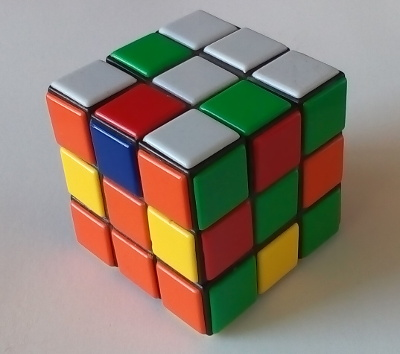
\includegraphics[scale=0.75]{\CURPATH/3solved.jpg}
\caption{Solved Rubik's cube as a pocket cube}
\end{figure}

\subsubsection{Some discussion}

\url{https://news.ycombinator.com/item?id=15214439},\\
\url{https://www.reddit.com/r/compsci/comments/6zb34i/solving_pocket_rubiks_cube_222_using_z3_and_sat/},\\
\url{https://www.reddit.com/r/Cubers/comments/6ze3ua/theory_dennis_yurichev_solving_pocket_rubiks_cube/}.

